\documentclass[a4paper]{report}
\usepackage[14pt]{extsizes}
\usepackage[utf8]{inputenc}
\usepackage[english,russian]{babel}
\usepackage[OT1]{fontenc}
\usepackage{setspace, amsmath}
\usepackage{amsfonts}
\usepackage{amssymb}
\usepackage[left=20mm, top=10mm, right=15mm, bottom=20mm, nohead, footskip=10mm]{geometry}
\usepackage{gensymb}

\usepackage{graphicx} 
\graphicspath{{images/}}
\DeclareGraphicsExtensions{.pdf,.png,.jpg}

\renewcommand{\theenumi}{\arabic{enumi}}
\renewcommand{\labelenumi}{\arabic{enumi}}
\renewcommand{\theenumii}{.\arabic{enumii}}
\renewcommand{\labelenumii}{\arabic{enumi}.\arabic{enumii}.}
\renewcommand{\theenumiii}{.\arabic{enumiii}}
\renewcommand{\labelenumiii}{\arabic{enumi}.\arabic{enumii}.\arabic{enumiii}.}
\usepackage{indentfirst}
\usepackage{fontspec}
\setmainfont{Times New Roman}

\begin{document}
\chapter{Изучение алгоритмов блочного и поточного шифрования данных}
\section{Алгоритмы блочного шифрования данных}
\subsection{Определение блочного шифра}
Блочный шифр — разновидность симметричного шифра, оперирующего группами бит фиксированной длины — блоками, характерный размер которых меняется в пределах 64‒256 бит. Если исходный текст (или его остаток) меньше размера блока, перед шифрованием его дополняют. Фактически, блочный шифр представляет собой подстановку на алфавите блоков, которая, как следствие, может быть моно- или полиалфавитной. Блочный шифр является важной компонентой многих криптографических протоколов и широко используется для защиты данных, передаваемых по сети.

Блочный шифр способен зашифровать одним ключом одно или несколько сообщений суммарной длиной больше, чем длина ключа. От поточных шифров работа блочного отличается обработкой бит группами, а не потоком. При этом блочные шифры медленнее поточных. Симметричные системы обладают преимуществом над асимметричными в скорости шифрования, что позволяет им оставаться актуальными, несмотря на более слабый механизм передачи ключа (получатель должен знать секретный ключ, который необходимо передать по уже налаженному зашифрованному каналу. В то же время, в асимметричных шифрах открытый ключ, необходимый для шифрования, могут знать все, и нет необходимости в передаче ключа шифрования).

К достоинствам блочных шифров относят сходство процедур шифрования и расшифрования, которые, как правило, отличаются лишь порядком действий. Это упрощает создание устройств шифрования, так как позволяет использовать одни и те же блоки в цепях шифрования и расшифрования. 
\newpage Гибкость блочных шифров позволяет использовать их для построения других криптографических примитивов: генератора псевдослучайной последовательности, поточного шифра, имитовставки и криптографических хешей.

\subsection{Структура блочного шифра}
Блочный шифр состоит из двух парных алгоритмов: шифрования и расшифрования. Оба алгоритма можно представить в виде функций. Функция шифрования E (encryption) на вход получает блок данных M (message) размером n бит и ключ K (key) размером k бит и на выходе отдает блок шифротекста C (cipher) размером n бит:

~

$E_K(M) := E(K,M) : \{0,1\}^k \times \{0,1\}^n \to \{0,1\}^n.$

~

Для любого ключа K, $E_K$ является биективной функцией (перестановкой) на множестве n-битных блоков. Функция расшифрования D (decryption) на вход получает шифротекст C, ключ K и на выходе отдает M:

~

$D_K(C) := D(K,C) : \{0,1\}^k \times \{0,1\}^n \to \{0,1\}^n,$

~

являясь, при этом, обратной к функции шифрования:

~

$D = E^{-1},$
\medskip

$\forall K: D_K(E_K(M)) = M$
\medskip

$E_K(D_K(C)) = C.$

~

Заметим, что ключ, необходимый для шифрования и дешифрования, один и тот же — следствие симметричности блочного шифра.

\section{Алгоритм шифрования DES}
Алгоритм шифрования данных DES (Data Encryption Standard) был опублико­ван в 1977 году. Является официальным стандартом США. Блочный симметричный алгоритм DES пока остается наиболее распространенным алгоритмом, используемым в системах защиты коммерческой информации.

\subsection{Принцип работы DES}

Алгоритм DES состоит из чередующейся последовательности перестановок и подстановок. Алгоритм DES осуществляет шифрование 64-битовых блоков данных с помощью 64-битового ключа, в котором значащими являются 56 бит (остальные 8 – проверочные биты для контроля четности).


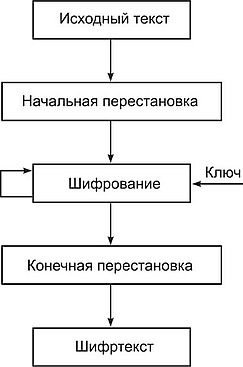
\includegraphics[scale=1.4]{DES}
{\centering{\newline Рис. 1.2.1.1 Обобщенная схема шифрования в алгоритме DES}\\}

~

Процесс шифрования в блочном алгоритме DES (рис. 1.2.1) заключается в начальной перестановке битов 64-битового блока, шестнадцати циклах (раундах) шифрования и, наконец, в конечной переста­новке битов. Расшифрование в DES является операцией, обратной шифрованию, и выполняется путем повторения операций шифрования в обратной последовательности.

~

\subsubsection{Процесс зашифрования}
Исходный текст $T$ (блок 64 бит) преобразуется c помощью начальной перестановки $IP$ которая определяется таблицей 1.2.1:

~

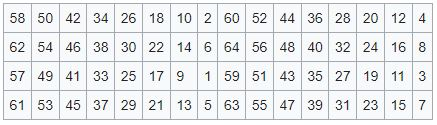
\includegraphics[scale=1.1]{табл}
{\centering{\newline Таблица 1.2.1.1 Начальная перестановка IP}\\}

~

По таблице первые 3 бита результирующего блока $IP(T)$ после начальной перестановкиявляются битами 58, 50, 42 входного блока , а его 3 последние бита являются битами 23, 15, 7 входного блока.

Полученный после начальной перестановки 64-битовый блок $IP(T)$ участвует в 16 циклах преобразования Фейстеля.

Преобразования Фейстеля- это преобразование над векторами (блоками), представляющими собой левую и правую половины регистра сдвига. В алгоритме DES используются прямое преобразование сетью Фейстеля в шифровании и обратное преобразование сетью Фейстеля в расшифровании.

~

16 циклов преобразования Фейстеля:

~

Разбить $IP(T)$ на две части $L_0, R_0$, где $L_0, R_0$ — соответственно 32 старших битов и 32 младших битов блока $T_{0} IP(T)$ = $L_0 R_0$

Пусть $T_{i-1}=L_{i-1}R_{i-1}$ результат (i-1) итерации, тогда результат i-ой итерации $T_{i}=L_{i}R_{i}$ определяется:

~

$L_i = R_{i-1}$ \\
$R_{i}=L_{i-1}\oplus f(R_{i-1},k_{i})$ 

~

Левая половина $L_{i}$ равна правой половине предыдущего вектора $L_{i-1}R_{i-1}$.\\ А правая половина $R_i$ — это битовое сложение $L_{i-1}$ и $f(R_{i-1},k_{i})$ по модулю 2.

~

В 16-циклах преобразования Фейстеля функция f играет роль шифрования.

Аргументами функции $f$ являются 32-битовый вектор $R_{i-1}$ и 48-битовый ключ $k_{i}$, который является результатом преобразования 56-битового исходного ключа шифра $k$. Для вычисления функции $f$ последовательно используются

\begin{enumerate}
\item функция расширения $E$
\item сложение по модулю 2 с ключом $k_{i}$
\item преобразование $S$, состоящее из 8 преобразований $S$-блоков ${S} _{1}$,${S} _{2}$,${S} _{3}$\ldots \ ${S} _{8}$
\item перестановка $P$
\end{enumerate}


\subsubsection{Генерирование ключей}
Ключи $k_{i}$ получаются из начального ключа $k$ (56 бит = 7 байтов или 7 символов в ASCII) следующим образом. Добавляются биты в позиции 8, 16, 24, 32, 40, 48, 56, 64 ключа $k$ таким образом, чтобы каждый байт содержал нечетное число единиц. Это используется для обнаружения ошибок при обмене и хранении ключей. Затем делают перестановку для расширенного ключа (кроме добавляемых битов 8, 16, 24, 32, 40, 48, 56, 64).

\subsubsection{Процесс расшифрования}
При расшифровании данных все действия выполняются в обратном порядке. В 16 циклах расшифрования, в отличие от шифрования c помощью прямого преобразования сетью Фейстеля, здесь используется обратное преобразование сетью Фейстеля.

~

$R_{i-1} = L_i$ \\
$L_{i-1} = R_i \oplus f(L_i,k_i)$

~

Ключ $k_{i}$, i=16,…,1, функция f, перестановка IP и $IP^{-1}$ такие же, как и в процессе шифрования. Алгоритм генерации ключей зависит только от ключа пользователя, поэтому при расшифровании они идентичны.


\subsection{Режимы использования DES}
DES может использоваться в четырёх режимах.

\begin{enumerate}
\item Режим электронной кодовой книги (ECB — Electronic Codebook): обычное использование DES как блочного шифра. Шифруемый текст разбивается на блоки, при этом каждый блок шифруется отдельно, не взаимодействуя с другими блоками (см. рис. 1.2.2.1)

~

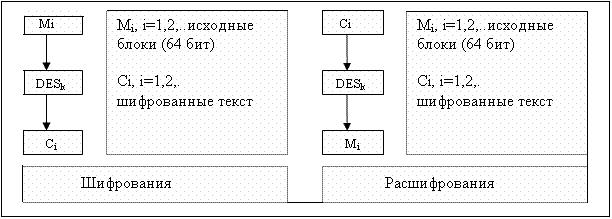
\includegraphics[scale=1.2]{ECB1}
{\centering{\newline Рис. 1.2.2.1 Режим электронной кодовой книги — ECB}\\}

~


\item Режим сцепления блоков шифротекста (СВС — Cipher Block Chaining)(см. рис. 1.2.2.2). Каждый очередной блок $M_{i}$ i>=1, перед зашифровыванием складывается по модулю 2 с предыдущим блоком зашифрованного текста $C_{i-1}$. Вектор $C_{0}$ — начальный вектор, он меняется ежедневно и хранится в секрете.

~

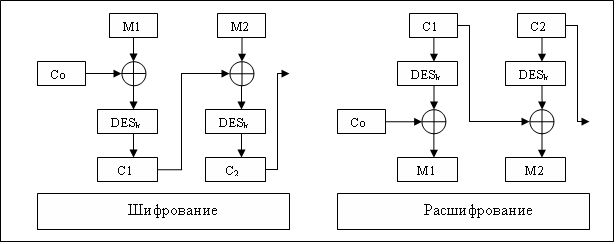
\includegraphics[scale=1.1]{CBC}
{\centering{\newline Рис. 1.2.2.2 Режим сцепления блоков — СВС}\\}

~

\item Режим обратной связи по шифротексту (Cipher Feedback) (см. рис.1.2.2.3). В режиме CFB вырабатывается блочная «гамма» $Z_{0},Z_{1},...,Z_{i}=DES_{k}(C_{i-1})$ $C_{i} = M_{i}\oplus Z_{i}$. Начальный вектор $C_{0}$ является синхропосылкой и предназначен для того, чтобы разные наборы данных шифровались по-разному с использованием одного и того же секретного ключа. Синхропосылка посылается получателю в открытом виде вместе с зашифрованным файлом. Алгоритм DES, в отличие от предыдущих режимов, используется только как шифрование (в обоих случаях).

~

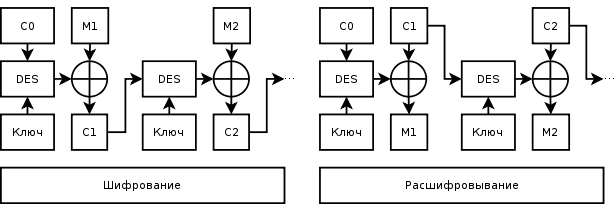
\includegraphics[scale=0.7]{CF}
{\centering{\newline Рис.1.2.2.3 Режим обратной связи по шифротексту — CFB}\\}

~

\item Режим обратной связи по выходу (OFB — Output Feedback) (см. Рис.10). В режиме OFB вырабатывается блочная «гамма» $Z_{0},Z_{1},...,Z_{i}=DES_{k}(Z_{i-1})C_{i}=M_{i}\oplus Z_{i}$ , i>=1. Режим также использует DES только как шифрование (в обоих случаях).

~

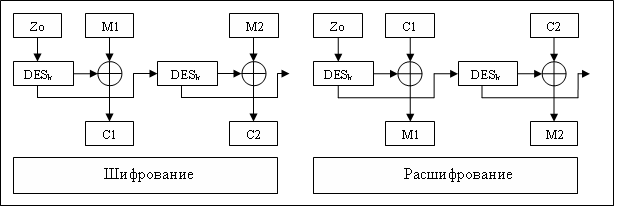
\includegraphics[scale=1.1]{OFB}
{\centering{\newline Рис. 1.2.2.4 Режим обратной связи по выходу — OFB}\\}
\end{enumerate}






\subsubsection{Достоинства и недостатки DES}
Основные достоинства алгоритма шифрования DES:
\begin{itemize}
\item относительная простота алгоритма обеспечивает высокую скорость\\ обработки;
\item для расшифровки сообщения, зашифрованного с помощью одного пакета программ, можно использовать любой другой пакет программ, соответствующий алгоритму DES;
\item криптостойкость алгоритма достаточна для защиты коммерческой \\ информации.
\end{itemize}

Также алгоритм DES имеет ряд существенных недостатков. Основные их них 
\begin{itemize}
\item битовые операции в узлах замены неэффективно реализуются программ­ным путем;
\item  короткая длина ключа (56 битов), что помогает организо­вать полный перебор;
\end{itemize}

\section{Алгоритм шифрования IDEA}
IDEA (англ. International Data Encryption Algorithm, международный алгоритм шифрования данных) — cимметричный блочный алгоритм шифрования данных, запатентованный швейцарской фирмой Ascom. Известен тем, что применяется в пакете программ шифрования PGP и в его свободной альтернативе GnuPG.

Первую версию алгоритма разработали в 1990 году Сюэцзя Лай и Джеймс Мэсси из Швейцарского института ETH Zürich в качестве замены DES и назвали ее PES (англ. Proposed Encryption Standard, предложенный стандарт шифрования). Затем, после публикации работ Бихама и Шамира по дифференциальному криптоанализу PES, алгоритм был улучшен с целью усиления криптостойкости и назван IPES (англ. Improved Proposed Encryption Standard, улучшенный предложенный стандарт шифрования). Через год его переименовали в IDEA.

~

IDEA использует 128-битный ключ и 64-битный размер блока. Открытый текст разбивается на блоки по 64 бит, если такое разбиение не возможно, используются различные режимы шифрования.Каждый исходный незашифрованный 64-битный блок делится на четыре подблока по 16 бит каждый, так как все алгебраические операции, использующиеся в процессе шифрования, совершаются над 16-битными числами. Для шифрования и расшифрования IDEA использует один и тот же алгоритм.

~

Фундаментальным нововведением в алгоритме является использование операций из разных алгебраических групп, а именно:
\begin{itemize}
\item сложение по модулю $2^{16}$
\item умножение по модулю $2^{16}+1$
\item побитовое исключающее ИЛИ (XOR).
\end{itemize}

~

Эти три операции несовместимы в том смысле, что:
\begin{itemize}
\item никакие две из них не удовлетворяют дистрибутивному закону, то есть \\ $a*(b+c)\ <>\ (a*b)+(a*c)$
\item никакие две из них не удовлетворяют ассоциативному закону, то есть \\ $a+(b\oplus c)\ <>\ (a+b)\oplus c$
\end{itemize}

~

Применение этих трех операций затрудняет криптоанализ IDEA по сравнению с DES, который основан исключительно на операции исключающее ИЛИ, а также позволяет отказаться от использования S-блоков и таблиц замены. IDEA является модификацией сети Фейстеля.

\section{Алгоритм шифрования RC5}

RC5 (Ron’s Code 5 или Rivest’s Cipher 5) — это блочный шифр, разработанный Роном Ривестом из компании RSA Security с переменным количеством раундов, длиной блока и длиной ключа.
Он отличается простотой, быстротой (за счет использования только примитивных компьютерных операций, таких как XOR, shift и т. Д.) И использует меньше памяти.
Это расширяет сферу использования и упрощает переход на более сильный вариант алгоритма. 



Существует несколько различных вариантов алгоритма, в которых преобразования в «пол-раундах» классического RC5 несколько изменены. В классическом алгоритме используются три примитивных операции и их инверсии:
\begin{itemize}

\item сложение по модулю $\displaystyle 2^{w}$
\item побитовое исключающее ИЛИ (XOR)
\item операции циклического сдвига на переменное число бит $(x \lll y).$
\end{itemize}

Основным нововведением является использование операции сдвига на переменное число бит, не использовавшиеся в более ранних алгоритмах шифрования. Эти операции одинаково быстро выполняются на большинстве процессоров, но в то же время значительно усложняют дифференциальный и линейный криптоанализ алгоритма.

Шифрование по алгоритму RC5 состоит из двух этапов. Процедура расширения ключа и непосредственно шифрование. Для расшифрования выполняется сначала процедура расширения ключа, а затем операции, обратные процедуре шифрования. Все операции сложения и вычитания выполняются по модулю $\displaystyle 2^{w}$. 

\subsubsection{Параметры алгоритма}
Так как алгоритм RC5 имеет переменные параметры, то для спецификации алгоритма с конкретными параметрами принято обозначение \textbf{RC5-W/R/b}, где:
\begin{itemize}
\item W — половина длины блока в битах, возможные значения 16, 32 и 64. Для эффективной реализации величину W рекомендуют брать равным машинному слову. Например, для 32-битных платформ оптимальным будет выбор W=32, что соответствует размеру блока 64 бита.
\item R — число раундов, возможные значения от 0 до 255. Увеличение числа раундов обеспечивает увеличение уровня безопасности шифра. Так, при R=0 информация шифроваться не будет. Также алгоритм RC5 использует таблицу расширенных ключей размера $\displaystyle 2(R+1)$ слов, которая получается из ключа заданного пользователем.
\item b — длина ключа в байтах, возможные значения от 0 до 255.
\end{itemize} 


\subsubsection{Расширение ключа}
Перед непосредственно шифрованием или расшифрованием данных выполняется процедура расширения ключа. Процедура генерации ключа состоит из четырёх этапов: 

\begin{itemize}

\item Генерация констант
\item Разбиение ключа на слова
\item Построение таблицы расширенных ключей
\item Перемешивание

\end{itemize}

\textbf{Генерация констант}

Для заданного параметра $W$ генерируются две псевдослучайные величины используя две математические константы: $e$ (экспонента) и $f$ (Золотое сечение).

$Q_w \leftarrow \textrm{Odd}((f − 1)\cdot 2^w)$

$P_w \leftarrow \textrm{Odd}((e − 2)\cdot 2^w)$

$\textrm{Odd()}$ - округление до ближайшего нечетного целого.

\textbf{Разбиение ключа на слова}

На этом этапе происходит копирование ключа $K_0 … K_{b − 1}$ в массив слов $L_0… L_{c − 1}$, где $c = b / u$, где $u = W / 8$, то есть, количество байт в слове.

Если $b$ не кратен $W / 8$, то $L$ дополняется нулевыми битами до ближайшего большего размера $c$, кратного $W / 8$.

В случае если $b = c = 0$, то мы устанавливаем значение $c = 1$, а $L_0 = 0$.

\textbf{Построение таблицы расширенных ключей}

На этом этапе происходит построение таблицы расширенных ключей $S_0 … S_{2 ∗ ( R + 1 ) − 1}$, которое выполняется следующим образом: 

$S_{0}=P_{w}$

$S_{i+1}=S_i+Q_w$

\textbf{Перемешивание}

Циклически N раз выполняются следующие действия:

${\displaystyle G=S_{i}=(S_{i}+G+H)\lll 3}$

${\displaystyle H=L_{j}=(L_{j}+G+H)\lll (G+H)}$

${\displaystyle i=(i+1)\mod (2(R+1))}$

${\displaystyle j=(j+1)\mod c}$,

$G, H, i, j$ — временные переменные, начальные значения которых равны 0. Количество итераций цикла N — это максимальное из двух значений $3 ∗ c$ и $(3 \cdot 2 \cdot (R + 1))$ 

\subsubsection{Шифрование}
Перед первым раундом выполняются операции наложения расширенного ключа на шифруемые данные:

$A=(A+S_0) \bmod {2^{w}}$

$B=(B+S_1)\bmod {2^{w}}$

В каждом раунде выполняются следующие действия: 

$A=((A\oplus B)\lll B)+S_{2i}$

$B=((B\oplus A)\lll A)+S_{2i+1}$

\subsubsection{Расшифрование}

Для Расшифрования данных используются обратные операции, то есть для $i = R, R − 1,...,1$ выполняются следующие раунды:

$B=((B-S_{2i+1})\ggg A)\oplus A$

$A=((A-S_{2i})\ggg B)\oplus B$

После выполнения всех раундов, исходное сообщение находится из выражения: 

$B=(B-S_1)\bmod {2^{w}}$

$A=(A-S_0)\bmod {2^{w}}$

\end{document}
